%%%%%%%%%%%%%%%%%%%%%%%%%%%%%%%%%%%%%%%%%
% Beamer Presentation
% LaTeX Template
% Version 1.0 (10/11/12)
%
% This template has been downloaded from:
% http://www.LaTeXTemplates.com
%
% License:
% CC BY-NC-SA 3.0 (http://creativecommons.org/licenses/by-nc-sa/3.0/)
%
%%%%%%%%%%%%%%%%%%%%%%%%%%%%%%%%%%%%%%%%%

%----------------------------------------------------------------------------------------
%	PACKAGES AND THEMES
%----------------------------------------------------------------------------------------

\documentclass{beamer}

\mode<presentation> {

	% The Beamer class comes with several default slide themes
	%, which changes the colors and layouts of slides. Below is a list
	% of all the themes, comment on each to see what they look like.

	%\usetheme{default}
	%\usetheme{AnnArbor}
	%\usetheme{Antibes}
	%\usetheme{Bergen}
	%\usetheme{Berkeley}
	%\usetheme{Berlin}
	%\usetheme{Boadilla}
	%\usetheme{CambridgeUS}
	%\usetheme{Copenhagen}
	%\usetheme{Darmstadt}
	%\usetheme{Dresden}
	%\usetheme{Frankfurt}
	%\usetheme{Goettingen}
	%\usetheme{Hannover}
	%\usetheme{Ilmenau}
	%\usetheme{JuanLesPins}
	%\usetheme{Luebeck}
	%\usetheme{Madrid}
	%\usetheme{Malmoe}
	%\usetheme{Marburg}
	%\usetheme{Montpellier}
	%\usetheme{PaloAlto}
	%\usetheme{Pittsburgh}
	\usetheme{Rochester}
	%\usetheme{Singapore}
	%\usetheme{Szeged}
	%\usetheme{Warsaw}

	% As well as themes, the Beamer class has several color themes
	% for any slide theme. Uncomment each of these, in turn, to see how it
	% changes the colors of your current slide theme.

	%\usecolortheme{albatross}
	\usecolortheme{beaver}
	%\usecolortheme{beetle}
	%\usecolortheme{crane}
	%\usecolortheme{dolphin}
	%\usecolortheme{dove}
	%\usecolortheme{fly}
	%\usecolortheme{lily}
	%\usecolortheme{orchid}
	%\usecolortheme{rose}
	%\usecolortheme{seagull}
	%\usecolortheme{seahorse}
	%\usecolortheme{whale}
	%\usecolortheme{wolverine}

	%\setbeamertemplate{footline} % To remove the footer line in all slides, uncomment this line
	%\setbeamertemplate{footline}[page number] % To replace the footer line in all slides with a simple slide count, uncomment this line

	%\setbeamertemplate{navigation symbols}{} % To remove the navigation symbols from the bottom of all slides, uncomment this line
}

\usepackage{graphicx} % Allows including images
\usepackage{booktabs} % Allows the use of \toprule, \midrule and \bottomrule in tables
% \titlegraphic{\includegraphics[height=2cm]{校徽}} % 插入校徽

\usepackage{ragged2e}
\justifying\let\raggedright\justifying %两端对齐

\usepackage{fontspec}
\setsansfont{Calibri}[
    Path=Font/,
    Scale=0.9,
    Extension = .ttf,
    UprightFont=*-Regular,
    BoldFont=*-Bold,
    ItalicFont=*-Italic,
    BoldItalicFont=*-BoldItalic
    ]
\usepackage{unicode-math}
\setmathfont{Libertinus Math} % 使用默认的数学字体或你偏好的数学字体 Latin Modern Math

%----------------------------------------------------------------------------------------
%	TITLE PAGE
%----------------------------------------------------------------------------------------

\title[Asset Pricing]{\textbf{Asset Pricing}} % The short title appears at the bottom of every slide, and the full title is only on the title page

\subtitle{1. Overview}

\author[Cheng Hang]{Cheng Hang} % Your name
\institute[DUFE] % Your institution, as it will appear on the bottom of every slide, may shorthand to save space
{School of Fintech \\
	Dongbei University of Finance \& Economics \\ % Your institution for the title page
	\medskip
	\textbf{chenghangch@qq.com}% Your email address
}
\date{\today} % Date, can be changed to a custom date

\AtBeginSection[]
{
	\begin{frame}{Content}
		\tableofcontents[sectionstyle=show/shaded,subsectionstyle=show/shaded/hide] %这几个参数我也不知道该如何准确地解释，反正它们最终的效果是突出显示当前章节，而其它章节都进行了淡化处理
		\addtocounter{framenumber}{-1}  %目录页不计算页码
	\end{frame}
}

%----------------------------------------------------------------------------------------
%	Begin
%----------------------------------------------------------------------------------------

\begin{document}

	\begin{frame}
		\titlepage % Print the title page as the first slide
	\end{frame}

	%\begin{frame}
	%\frametitle{Overview} % Table of contents slide, comment this block out to remove it
	%\tableofcontents % Throughout your presentation, if you choose to use \section{} and \subsection{} commands, these will automatically be printed on this slide as an overview of your presentation
	%\end{frame}

	%----------------------------------------------------------------------------------------
	%	PRESENTATION SLIDES
	%----------------------------------------------------------------------------------------



\section{Instructor}

\begin{frame}{Instructor}
	\begin{itemize}
		\item Name: Cheng Hang (A.P)
		\item Bachelor: Mathematics (BUAA)
		\item Master: Finance (DUFE)
		\item Ph.D: Financial Engineering (DUFE)
	\end{itemize}
\end{frame}

\begin{frame}{Contact Information}
	\begin{itemize}
		\item Academic interests (Focus on Empirical Research): 
		\begin{itemize}
		  \item Time Series Forecasting
            \item Anomalies/Pricing Factors
            \item Climate Finance
            \item High-Frequency Trading Data
            \item ...
		\end{itemize}
		\item Website: \href{https://chenghang.work}{\textcolor{blue}{https://chenghang.work}}
		\item Office: Room 347, Zi Nan Building
		\item Email: chenghangch@qq.com
	\end{itemize}
\textbf{If you have any questions, please don't hesitate to contact me.}
\end{frame}

\section{Course Description}

\begin{frame}{Learning Objectives}
By the end of this course, you should be able to:
\begin{enumerate}
	\item \textbf{Understand} the theoretical foundations of asset pricing models, from CAPM to multi-factor models
	\item \textbf{Apply} econometric methods to test asset pricing theories
	\item \textbf{Replicate} classic empirical findings in asset pricing literature
	\item \textbf{Critically evaluate} academic papers in top finance journals
	\item \textbf{Conduct} original empirical research using Chinese market data
	\item \textbf{Communicate} your research findings effectively in written and oral form
\end{enumerate}
\end{frame}

\begin{frame}{Why Study Asset Pricing?}
	\begin{itemize}
		\item \textbf{Intellectual Foundation}: Asset pricing is the core of modern finance theory
		\begin{itemize}
			\item Connects economics, statistics, and real-world markets
			\item Provides a framework for understanding risk and return
		\end{itemize}
		\item \textbf{Practical Applications}:
		\begin{itemize}
			\item Portfolio management and asset allocation
			\item Risk management and derivatives pricing
			\item Corporate finance decisions (cost of capital)
			\item Regulatory policy (market efficiency)
		\end{itemize}
		\item \textbf{Research Opportunities}:
		\begin{itemize}
			\item Active area with many open questions
			\item China's market offers unique research opportunities
			\item Growing importance of machine learning methods
		\end{itemize}
	\end{itemize}
\end{frame}

\begin{frame}{Historical Development of Asset Pricing Theory}
\small{
\begin{center}
\begin{tabular}{cl}
	\toprule
	\textbf{Year} & \textbf{Milestone} \\
	\midrule
	1952 & \href{https://doi.org/10.1111/j.1540-6261.1952.tb01525.x}{\textcolor{blue}{Markowitz: Mean-Variance Portfolio Theory}} \\
	1958 & \href{https://www.jstor.org/stable/1809766}{\textcolor{blue}{Modigliani-Miller: Capital Structure Irrelevance}} \\
	1964 & \href{https://doi.org/10.1111/j.1540-6261.1964.tb02865.x}{\textcolor{blue}{Sharpe: Capital Asset Pricing Model (CAPM)}} \\
	1970 & \href{https://doi.org/10.2307/2325486}{\textcolor{blue}{Fama: Efficient Market Hypothesis}} \\
	1973 & \href{https://doi.org/10.1086/260062}{\textcolor{blue}{Black-Scholes-Merton: Option Pricing}} \\
	1976 & \href{https://doi.org/10.1016/0022-0531(76)90046-6}{\textcolor{blue}{Ross: Arbitrage Pricing Theory (APT)}} \\
	1982 & \href{https://doi.org/10.2307/1912775}{\textcolor{blue}{Hansen: GMM Estimation}} \\
	1985 & \href{https://doi.org/10.1016/0304-3932(85)90061-3}{\textcolor{blue}{Mehra-Prescott: Equity Premium Puzzle}} \\
	1993 & \href{https://doi.org/10.1016/0304-405X(93)90023-5}{\textcolor{blue}{Fama-French: Three-Factor Model}} \\
	2004 & \href{https://doi.org/10.1111/j.1540-6261.2004.00670.x}{\textcolor{blue}{Bansal-Yaron: Long-Run Risk Model}} \\
	2015 & \href{https://doi.org/10.1093/rfs/hhu068}{\textcolor{blue}{Hou-Xue-Zhang: q-Factor Model}} \\
	2020 & \href{https://doi.org/10.1093/rfs/hhaa009}{\textcolor{blue}{Gu-Kelly-Xiu: Machine Learning in Asset Pricing}} \\
	\bottomrule
\end{tabular}
\end{center}
}
\end{frame}

\begin{frame}{Main Theme}
	We discuss each topic in three respects:
	\begin{itemize}
		\item commonly used empirical methodologies
		\item main empirical findings
		\item the relation between empirics and theories
	\end{itemize}
\end{frame}

\begin{frame}{Prerequisites}
	\begin{itemize}
		\item Graduate-level courses in finance and econometrics
		\item Statistical packages: \alert{Python}, \alert{R}, SAS, MATLAB, STATA, …
		\item Access to CSMAR, Wind, and RESSET database
	\end{itemize}
\end{frame}

\begin{frame}{Books}
	\begin{itemize}
		\item Campbell, John Y, Andrew Wen-Chuan Lo, and Archie Craig MacKinlay, 1997. \alert{\textbf{The Econometrics of Financial Markets}}
		\item Cochrane, John H., 2005.\alert{ \textbf{Asset Pricing}}.
		\item Bali, Turan, Robert Engle, and Scott Murray, 2017, \alert{\textbf{Empirical Asset Pricing: The cross-section of stock returns: An overview}}
		\item Campbell, John Y, 2017. \alert{\textbf{Financial Decisions and Markets: A course in asset pricing}}
	\end{itemize}
\end{frame}

\begin{frame}{Additional Resources}
	\begin{itemize}
		\item \textbf{Useful Survey Papers}:
		\begin{itemize}
			\item \href{https://doi.org/10.1146/annurev-financial-110112-120833}{\textcolor{blue}{Nagel (2013)}}: Empirical Cross-Sectional Asset Pricing
			\item \href{https://doi.org/10.1093/rfs/hhv059}{\textcolor{blue}{Harvey, Liu, and Zhu (2016)}}: ... and the Cross-Section of Expected Returns
			\item \href{https://doi.org/10.1146/annurev-financial-101521-104735}{\textcolor{blue}{Giglio, Kelly, and Xiu (2022)}}: Factor Models, Machine Learning...
		\end{itemize}
		\item \textbf{Online Resources}:
		\begin{itemize}
			\item \href{https://www.openassetpricing.com/}{\textcolor{blue}{Open Source Asset Pricing}} (Andrew Y. Chen)
			\item \href{https://wrds-www.wharton.upenn.edu/}{\textcolor{blue}{WRDS}} (Wharton Research Data Services)
			\item \href{https://mba.tuck.dartmouth.edu/pages/faculty/ken.french/data_library.html}{\textcolor{blue}{Kenneth French Data Library}}
		\end{itemize}
		\item \textbf{Chinese Market Data}:
		\begin{itemize}
			\item \href{https://www.resset.cn/}{\textcolor{blue}{RESSET Database}}
			\item \href{https://www.gtarsc.com/}{\textcolor{blue}{CSMAR Database}}
		\end{itemize}
	\end{itemize}
\end{frame}

\begin{frame}{Frontier Research}
	\begin{itemize}
		\item \href{https://www.nber.org/programs-projects/programs-working-groups/asset-pricing}{\textcolor{blue}{NBER Asset Pricing Working Papers}}
		\item \href{https://papers.ssrn.com/sol3/DisplayAbstractSearch.cfm}{\textcolor{blue}{SSRN}}
		\item Programs of major finance conferences: \href{https://editorialexpress.com/conference/AFA2022/program/AFA2022.html}{\textcolor{blue}{AFA}}, WFA, EFA, …
		\item Research websites of active asset pricing researchers: \href{https://www.johnhcochrane.com/}{\textcolor{blue}{John H. Cochrane}}, \href{http://homepages.uc.edu/~guohu/}{\textcolor{blue}{Hui Guo}},\href{https://apps.olin.wustl.edu/faculty/zhou/}{\textcolor{blue}{Guofu Zhou}},\href{https://theinvestmentcapm.com/index.html}{\textcolor{blue}{Lu Zhang}}
		\item Journals:
          \begin{enumerate}
              \item \href{https://onlinelibrary.wiley.com/journal/15406261}{\textcolor{blue}{Journal of Finance}} \textcolor{red}{(T1)}
              \item \href{https://academic.oup.com/rfs/issue}{\textcolor{blue}{Review of Financial Studies}} \textcolor{red}{(T1)}
              \item \href{https://www.sciencedirect.com/journal/journal-of-financial-economics}{\textcolor{blue}{Journal of Financial Economics}} \textcolor{red}{(T1)}
              \item \href{https://www.cambridge.org/core/journals/journal-of-financial-and-quantitative-analysis}{\textcolor{blue}{Journal of Financial and Quantitative Analysis}} \textcolor{red}{(T2)}
              \item \href{https://academic.oup.com/rof}{\textcolor{blue}{Review of Finance}} \textcolor{red}{(T2)}
              \item \href{https://www.sciencedirect.com/journal/journal-of-banking-and-finance}{\textcolor{blue}{Journal of Banking \& Finance}} \textcolor{red}{(T2)}
              \item \href{https://academic.oup.com/raps/issue}{\textcolor{blue}{The Review of Asset Pricing Studies}} \textcolor{red}{(B)}
          \end{enumerate}
	\end{itemize}
\end{frame}

\begin{frame}{Grading}
	\begin{itemize}
		\item Homework (30\%)
		\item Final Assignments (70\%)
	\end{itemize}

This will be a demanding course, and I expect you to work \textbf{VERY HARD}. By the end of the course, you are expected to be familiar with relevant economic issues and have the skills required for doing empirical research. The ultimate objective is that you should be able to conduct the original research in empirical asset pricing.

\end{frame}

\section{Introduction}


\begin{frame}{Nobel Memorial Prize in Economic Sciences}
    \begin{itemize}
	\item 1990: \alert{``for their pioneering work in the theory of financial economics''}
	\begin{figure}
		\centering
		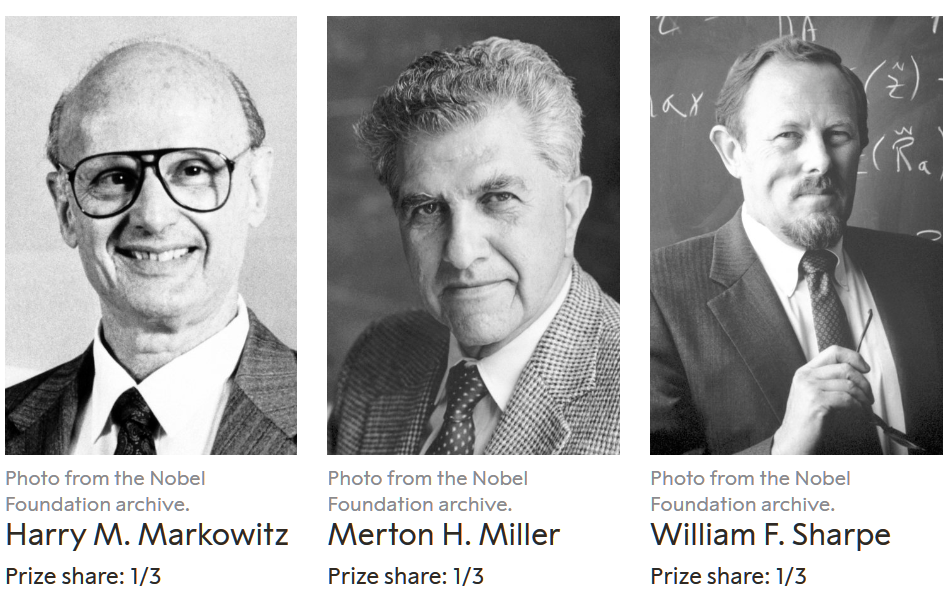
\includegraphics[width=1\linewidth]{Files/1990Nobel.png}
	  \end{figure}
% \begin{itemize}
% 	\item The contribution for which Harry Markowitz received the Economic Sciences Prize was first published in the essay Portfolio Selection (1952) and later in his book Portfolio Selection: Efficient Diversification (1959). The theory of portfolio selection was originally normative for investment managers, i.e., a theory for the optimal investment of wealth in assets that differ concerning their expected return and risk. His theory evolved into a foundation for further research in financial economics.
% 	\item Merton Miller collaborated with his colleague Franco Modigliani (Economic Sciences Prize 1985) on the paper The Cost of Capital, Corporate Finance and the Theory of Investment. The Modigliani-Miller theorem explains the relationship between a company's capital asset structure and dividend policy and its market value and cost of capital. The theorem demonstrates that how a manufacturing company funds its activities is less important than the profitability of those activities.
% 	\item William Sharpe's research yielded the Capital Asset Pricing Model (CAPM) in a paper submitted in 1962. The CAPM theory is based on the earlier work of fellow Laureate Harry Markowitz. The model makes it possible to judge a portfolio's performance by the amount of risk inherent in such investments and helps managers decide when potential return is worth the risks of the investment.
% \end{itemize}
    \end{itemize}
\end{frame}

\begin{frame}{Nobel Memorial Prize in Economic Sciences}
    \begin{itemize}
	\item 1997: \alert{``for a new method to determine the value of derivatives''}
	\begin{figure}
	  \centering
	  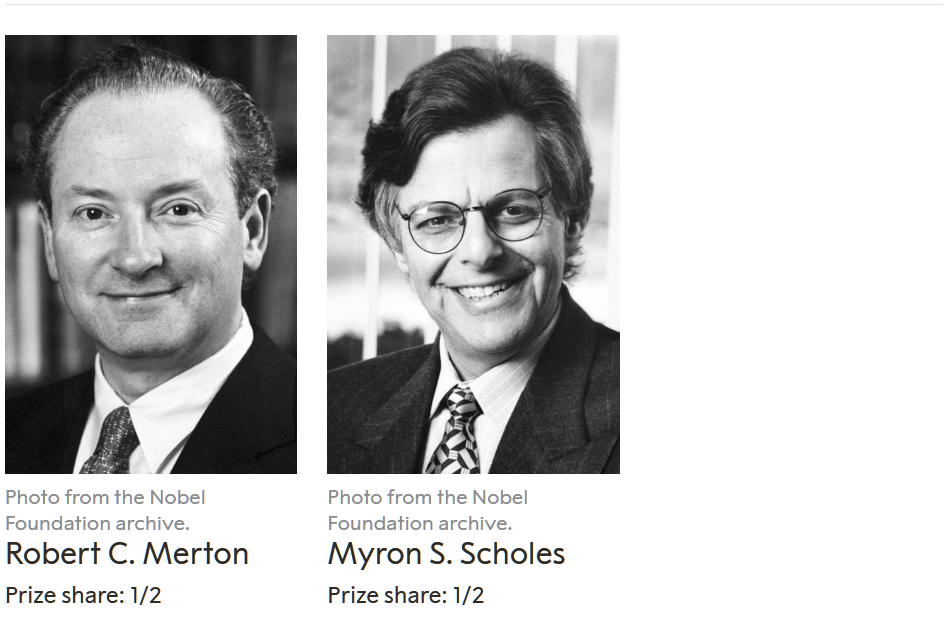
\includegraphics[width=1.01\linewidth]{Files/1997Nobel.png}
	\end{figure}
% \begin{itemize}
% 	\item Robert Merton is known for his work on finance theory and risk management, especially for his contribution to assessing the value of stock options and other derivatives. Merton used his background in mathematics to generalize the Black-Scholes formula, created by Myron Scholes and Fischer Black. By altering the formula, Merton allowed it to apply to other financial matters, such as mortgages and student loans.
% 	\item Myron Scholes is known for his work with colleague Fischer Black on the Black-Scholes option valuation formula, which made options trading more accessible by giving investors a benchmark for valuing. Scholes shared the Economic Sciences Prize with Robert Merton, who generalized the Black-Scholes formula to make it apply to other areas of finance. (Black died in 1995 and was ineligible for the Economic Sciences Prize.)
% \end{itemize}
    \end{itemize}
\end{frame}

\begin{frame}{Nobel Memorial Prize in Economic Sciences}
    \begin{itemize}
	\item 2013: \alert{``for their empirical analysis of asset price''}
	\begin{figure}
	  \centering
	  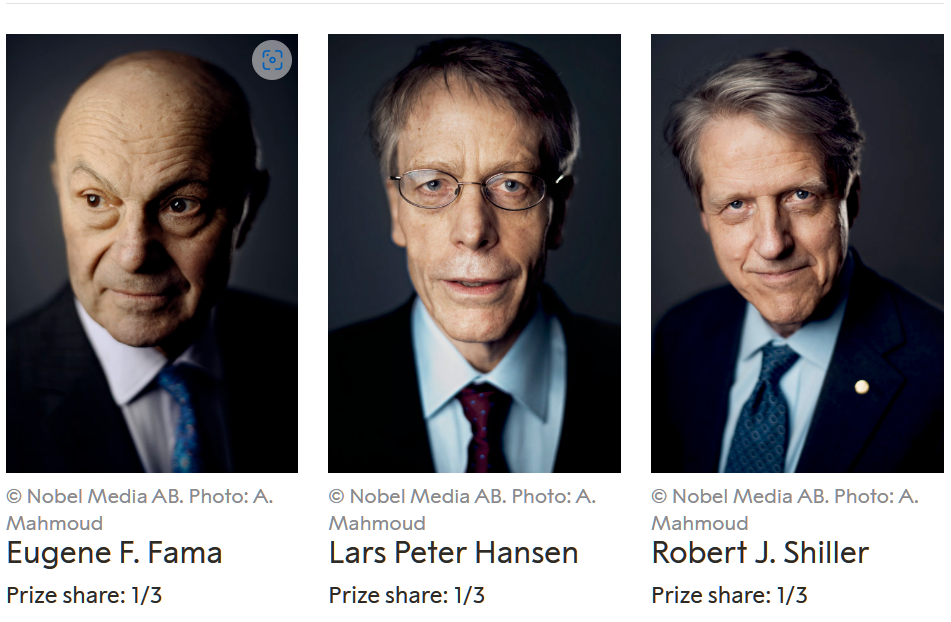
\includegraphics[width=1\linewidth]{Files/2013Nobel.png}
	\end{figure}
    \end{itemize}
\end{frame}

\begin{frame}{Nobel Memorial Prize in Economic Sciences}
\small{
	\begin{itemize}
		\item For many of us, the rise and fall of stock prices symbolizes economic development. In the 1960s, Eugene Fama demonstrated that stock price movements are impossible to predict in the short term and that new information affects prices almost immediately, which means that the market is efficient. The impact of Fama's results has extended beyond the field of research. For example, Fama's results influenced the development of index funds.
		\item Eugene Fama demonstrated that stock price movements are impossible to predict in the short term, while Robert Shiller discovered that stock prices can be predicted over a longer period. In 1982, Lars Peter Hansen developed a statistical method for testing this type of theory. He demonstrated that Shiller's results could not be fully explained within the then-current models, and Hansen's method is now used within all economics research.
		\item In the early 1980s, however, Robert Shiller discovered that stock prices can be predicted over a longer period, such as over several years. In contrast to the dominant perception, stock prices fluctuated much more than corporate dividends. Shiller's conclusion was, therefore, that the market is inefficient.
	 \end{itemize}}
\end{frame}


\begin{frame}{Nobel}
	\begin{figure}
		\centering
		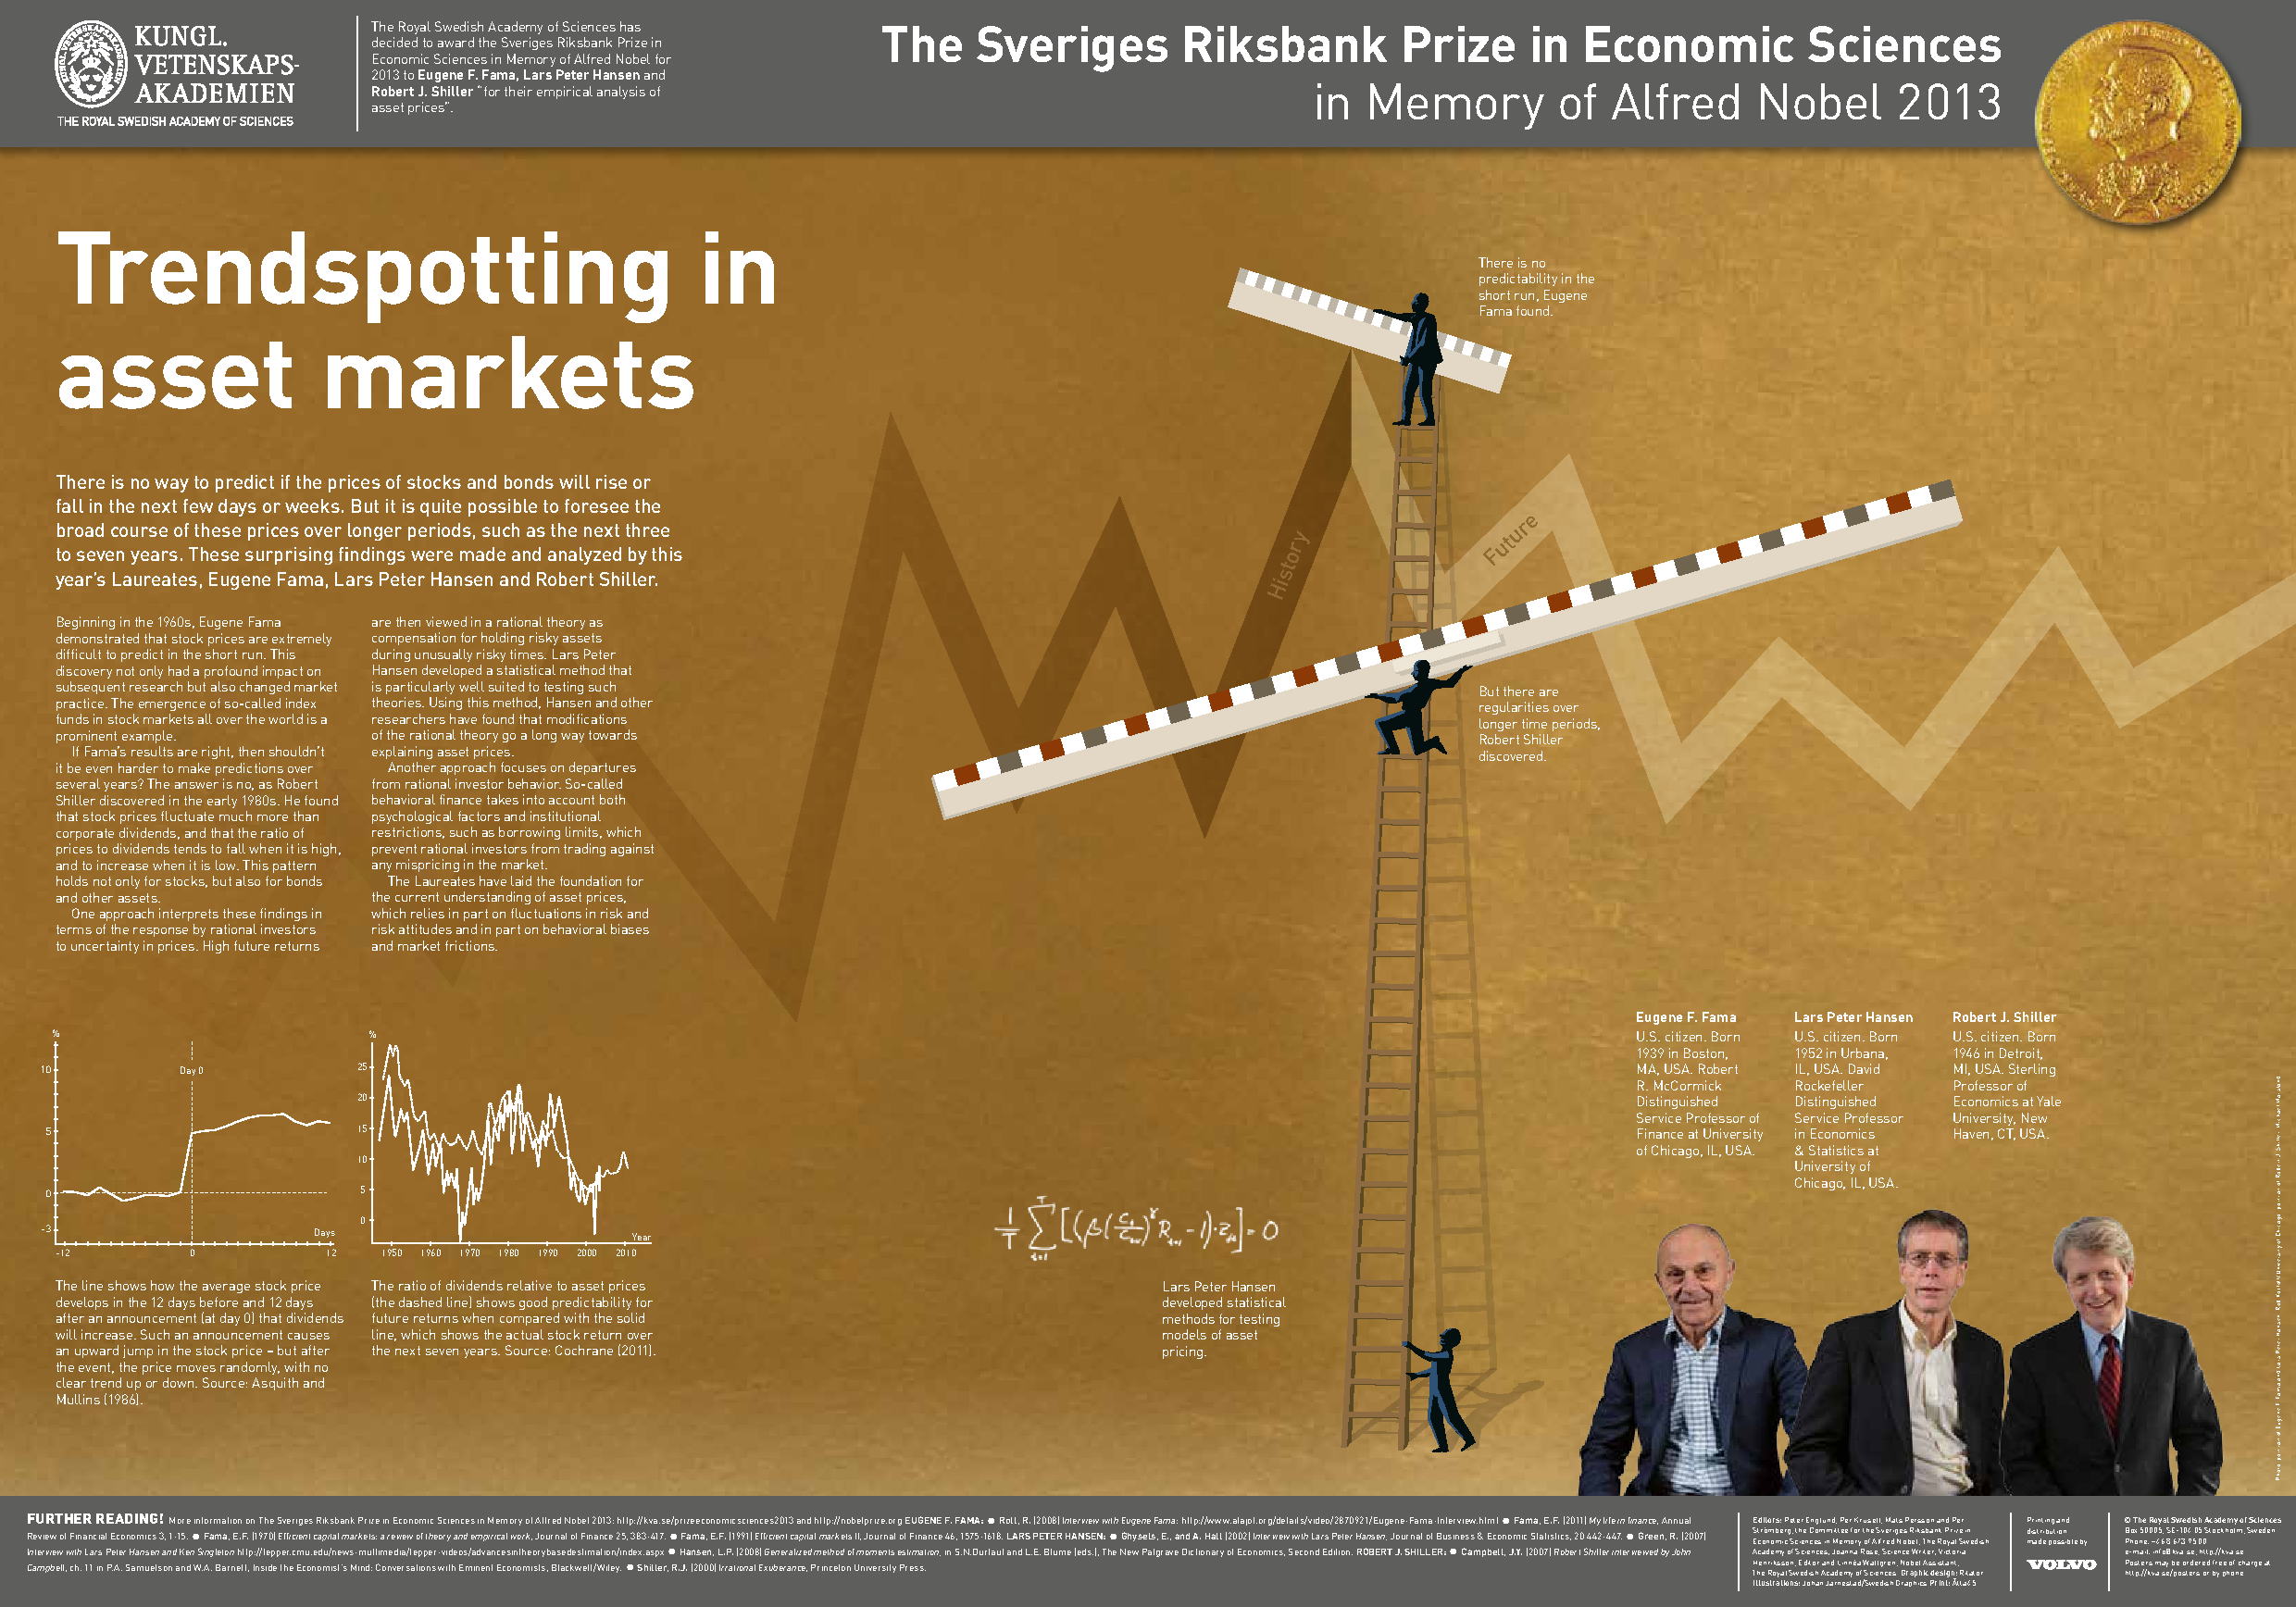
\includegraphics[width=1\linewidth]{Files/poster_economicsciences_web.pdf}
	\end{figure}
\end{frame}


\begin{frame}{Introduction}
	\begin{itemize}
		\item A big picture to guide you through the vast literature
		\begin{itemize}
			\item how selected topics are related to each other
			\item the evolution of asset pricing theories
			\item interesting issues (my personal view)
		\end{itemize}
		\item The overview
		\begin{itemize}
			\item is highly selective, focusing on consumption-based CAPM
			\item reflects strongly my own opinion
			\item Risk-Based Asset Pricing Theory
		\end{itemize}
		\item You should always try to
		\begin{itemize}
			\item form your own view based on sound reasoning
			\item be open-minded
			\item has a healthy dose of doubts
		\end{itemize}
\end{itemize}
\end{frame}

\begin{frame}{Main Theme: Time-Varying Risk Premium}
	\textbf{Discount Rates} (AFA Presidential Address by \href{https://doi.org/10.1111/j.1540-6261.2011.01671.x}{\textcolor{blue}{Cochrane (2011)}})
	\begin{itemize}
		\item Discount-rate variation is the \alert{central} organizing question of current asset-pricing research.
		\item Previously, we thought returns were unpredictable, with variations in price-dividend ratios due to variations in expected cash flows. Now, it seems all price-dividend variation corresponds to \textcolor{red}{discount-rate variation}.
		\item We also thought that the cross-section of expected returns came from the CAPM. \textcolor{red}{We have a zoo of new factors now}.
		\item Incorporating discount-rate variation affects finance applications, including portfolio theory, accounting, cost of capital, capital structure, compensation, and macroeconomics.
	\end{itemize}
\end{frame}

\section{Overview of Selected Topics}

\subsection{Essence of Asset Pricing}

\begin{frame}{How to price a risky asset, e.g., a stock or a bond?}
	\textbf{Essence} of Asset Pricing: Cash flows and discount rates
	\begin{align*}
		P_{t}=E_{t}\left(m_{t+1} *  \mathrm{payoff}_{t+1}\right)
	\end{align*}
$m_{t+1}$: stochastic discount factor or pricing kernel
\begin{align*}
	P_{t}=E_{t}\left[\sum_{i=1}^{\infty}\left(\frac{1}{1+R_{t+1}}\right)^{i} D_{t+i}\right]
\end{align*}
\end{frame}

\begin{frame}{The Central Equation of Asset Pricing}
	\textbf{All} asset pricing models can be written as:
	\begin{align*}
		1 = E_t[m_{t+1} \cdot R_{t+1}]
	\end{align*}
	where $m_{t+1}$ is the \alert{stochastic discount factor (SDF)}.
	
	\vspace{10pt}
	\textbf{Equivalent representations}:
	\begin{itemize}
		\item \textbf{Risk-neutral pricing}: $P_t = \frac{1}{R_f} E^Q_t[X_{t+1}]$
		\item \textbf{Beta pricing}: $E[R_i] - R_f = \beta_i \lambda$
		\item \textbf{Mean-variance frontier}: Efficient portfolios
	\end{itemize}
	
	\vspace{10pt}
	\textbf{Key insight}: Different models are different stories about $m_{t+1}$
	\begin{itemize}
		\item CAPM: $m_{t+1} = a + b \cdot R_{M,t+1}$
		\item C-CAPM: $m_{t+1} = \beta \left(\frac{C_{t+1}}{C_t}\right)^{-\gamma}$
		\item Multi-factor: $m_{t+1} = a + b_1 f_1 + b_2 f_2 + ...$
	\end{itemize}
\end{frame}

\begin{frame}{Essence of Asset Pricing}
	\textbf{The hurdles in asset pricing are really conceptual rather than mathematical (John H. Cochrane (2005), Preface).}

	\vspace{10pt}
	\textbf{Of course, Cochrane means that asset pricing is really about the identification of systematic risk or provides a good explanation about what had happened and, more importantly, prediction.}
\end{frame}

\begin{frame}{Essence of Asset Pricing}
	\begin{itemize}
		\item We want to ensure that assets are correctly priced.
		\item This is a VERY difficult task because SDF is unobservable.
		\item Efficient Market Hypothesis Testing:
		\begin{itemize}
			\item No arbitrage pricing: assets with identical cash flows have identical price
			\item We try to identify a unique SDF that prices all assets
			\item joint hypothesis problem: an SDF does not price all assets because
			\begin{enumerate}
				\item market is
				inefficient
				\item it is not the correct SDF
			\end{enumerate}
			\item Asset pricing is a scientific search for SDF analogous to physics.
		\end{itemize}
	\end{itemize}
\end{frame}

\subsection{EMH}

\begin{frame}{Efficient Market Hypothesis (EMH)}
	\begin{itemize}
		\item Financial market participants always try to beat the market. EMH suggests no free lunch
		\begin{itemize}
			\item Market is \textit{efficient} if price fully reflect all available information (\href{https://doi.org/10.2307/2325486}{\textcolor{blue}{Fama(1970)}})
			\item There is a tradeoff between risk and return
		\end{itemize}
		\item Limit of arbitrage: mispricing exists because it is costly to arbitrage
		\begin{itemize}
			\item Example: high idiosyncratic volatility stocks have higher expected returns
			because they have high information or arbitrage costs
		\end{itemize}
		\item Behavior-based (irrational) pricing: 
		     \begin{itemize}
			\item Example: investors are over-optimistic about growth or glamour stocks
			\item Investor sentiment is a belief about future cash flows and investment risks that is not justified by the facts at hand (\href{https://www.aeaweb.org/articles?id=10.1257/jep.21.2.129}{\textcolor{blue}{Baker and Wurgler (2007)}}, p.129)
		\end{itemize}
	\end{itemize}
\end{frame}

\begin{frame}{Three Forms of Market Efficiency}
	\href{https://doi.org/10.2307/2325486}{\textcolor{blue}{Fama (1970)}} classifies market efficiency into three forms:
	\begin{itemize}
		\item \textbf{Weak Form}: Prices reflect all past price information
		\begin{itemize}
			\item Implication: Technical analysis cannot earn excess returns
			\item Test: Autocorrelation of returns, runs tests
		\end{itemize}
		\item \textbf{Semi-Strong Form}: Prices reflect all publicly available information
		\begin{itemize}
			\item Implication: Fundamental analysis cannot earn excess returns
			\item Test: Event studies (earnings announcements, stock splits)
		\end{itemize}
		\item \textbf{Strong Form}: Prices reflect all information (public and private)
		\begin{itemize}
			\item Implication: Even insiders cannot earn excess returns
			\item Test: Performance of mutual funds, insider trading studies
		\end{itemize}
	\end{itemize}
	
	\vspace{5pt}
	\textbf{Modern view}: Markets are ``efficiently inefficient'' (\href{https://press.princeton.edu/books/hardcover/9780691166193/efficiently-inefficient}{\textcolor{blue}{Pedersen (2015)}})
\end{frame}


\begin{frame}{Efficient Market Hypothesis (EMH)}
	\begin{itemize}
		\item In the 1960s, EMH has been commonly interpreted as implying constant
		expected stock returns (\textcolor{red}{wrong}).
		\item Many authors have tested whether available information, e.g., past returns to forecast stock returns and found mixed results. However, they generally agree that markets were reasonably efficient in the sense that the documented stock return predictability is economically small.
		\item Yet there is a \textit{simple} and \textit{powerful} test by looking at \textbf{present value relation}.
	\end{itemize}
\end{frame}

\begin{frame}{Present-Value Relation with Constant Expected Returns}
\begin{equation*}
    \begin{aligned}
		1+R_{t+1}&=\frac{P_{t+1}+D_{t+1}}{P_{t}} \\
		P_{t}&=\frac{P_{t+1}+D_{t+1}}{1+R_{t+1}} \\
		P_{t}&=E_{t}\left(P_{t}\right)=E_{t}\left[\frac{P_{t+1}+D_{t+1}}{1+R_{t+1}}\right]\xrightarrow[E_t(R_{t+1})]{constant}E_{t}\left[\frac{\left(P_{t+1}\right)+D_{t+1}}{1+R}\right] \\
		&=E_{t}\left[\sum_{i=1}^{k} \frac{1}{(1+R)^{i}} D_{t+i}\right]+\underbrace{E_{t}[\frac{1}{(1+R)^{k}} P_{t+k}]}_{\simeq 0} (k\longrightarrow \infty) \\
		& = E_{t}\left[\sum_{i=1}^{\infty} \frac{1}{(1+R)^{i}} D_{t+i}\right]
    \end{aligned}
\end{equation*}
\end{frame}

\begin{frame}{Excess Volatility Puzzle}
	\begin{equation*}
		P_{t} = E_{t}\left[\sum_{i=1}^{\infty} \frac{1}{(1+R)^{i}} D_{t+i}\right]
	\end{equation*}
\begin{itemize}
	\item Null Hypothesis: If expected returns are constant, variation in dividends
	should fully explain variations in stock prices.
	\item \textbf{Excess Volatility Puzzle} (\href{http://www.jstor.org/stable/1802789}{\textcolor{blue}{Shiller (1981)}}): The present value relation falls apart
	in data because stock prices are much more volatile than dividends.
	\item Many researchers interpret excess stock price volatility as evidence of
	irrational pricing because stock prices do not reflect fundamentals.
	Shiller's findings pose a challenge to the efficient market hypothesis and
	inspire behavioral asset pricing models.
\end{itemize}
\end{frame}

\begin{frame}{Excess Volatility Puzzle}
	Excess volatility puzzle does not necessarily imply inefficient markets.
	\begin{itemize}
		\item It might reflect a time-varying risk premium.
		\item Shiller's findings inspire empirical research on time-series stock market
		return predictability.
		\item For many economists, discount-rate variation is the central organizing
		question of current asset-pricing research.
	\end{itemize}
\end{frame}

\begin{frame}{Excess Volatility Puzzle Reflects Time-Varying Risk Premium}
	\begin{itemize}
		\item \href{https://doi.org/10.2307/2233809}{\textcolor{blue}{Campebll (1991)}} and \href{http://www.jstor.org/stable/2962031}{\textcolor{blue}{Cochrane (1992)}} show that discount rate shocks account for most variance in stock prices
		\begin{itemize}
			\item More recent evidence suggests both shocks are important
		\end{itemize}
		\item The dividend yield should forecast stock market returns, especially over long horizons. (Empirical evidence by  \href{https://doi.org/10.1093/rfs/1.3.195}{\textcolor{blue}{Campebll and Shiller (1988)}}, \href{http://www.sciencedirect.com/science/article/pii/0304405X89900950}{\textcolor{blue}{Fama and French (1989)}}, among others, provides support for this view)
		\item \href{https://doi.org/10.1111/j.1540-6261.1991.tb04636.x}{\textcolor{blue}{Fama (1991)}} stresses that EMH does NOT necessarily imply constant expected returns
		\item We need a theory or story of time-varying expected returns
	\end{itemize}
\end{frame}

\subsection{Predictability Debate}
\begin{frame}{Predictability Debate}
	\begin{itemize}
		\item Skepticism
		\begin{itemize}
			\item \href{http://www.jstor.org/stable/40056859}{\textcolor{blue}{Welch and Goyal (2008)}}   investigate the variables that have been found to forecast stock returns in the empirical literature. None of them forecast
			stock returns in long samples, especially in the out-of-sample context.
			\item \href{https://doi.org/10.1093/rfs/hhl042}{\textcolor{blue}{Boudoukh, Richardson, and Whitelaw (2008)}} : Long-horizon
			regressions provide little information beyond short-horizon regressions.
		\end{itemize}
		\item Defense
		\begin{itemize}
			\item \href{https://doi.org/10.1093/rfs/hhm046}{\textcolor{blue}{Cochrane (2008)}} emphasizes that if expected returns are constant, stock
			prices should be much less volatile than we have observed in the data.
		\end{itemize}
	\end{itemize}
\end{frame}

\begin{frame}{Predictability Debate: Interpretation of New Evidence}
	\begin{itemize}
		\item The positive risk-return relation is \textbf{the first fundamental law of finance}.
		\item In \href{http://www.jstor.org/stable/2117530}{\textcolor{blue}{Campbell's ICAPM (1993)}}, if stock returns are predictable, expected returns are also determined by the covariance with discount-rate shocks.
        \begin{equation*}
            E_{t}\left(R_{M, t+1}\right)=\gamma \sigma_{M, t}^{2}+(\gamma-1) \beta_{M, D R} \sigma_{D R, t}^{2}
        \end{equation*}
		\item Empirical support: \href{https://doi.org/10.1111/j.1540-6261.2006.00877.x}{\textcolor{blue}{Guo and Whitelaw (2006)}}, \href{https://doi.org/10.1016/j.jfineco.2012.07.001}{\textcolor{blue}{Maio and Santa-Clara (2012)}}, \href{https://www.sciencedirect.com/science/article/pii/S0378426624000372}{\textcolor{blue}{Cheng, Guo and Shi (2024)}}
	\end{itemize}
\end{frame} 


\begin{frame}{Predictability Debate: Is There a Reconciliation?}
	The current debate focuses mainly on dividend yield
	\begin{itemize}
		\item A sufficient statistic for expected returns when market volatility is the only
		risk factor: \href{https://doi.org/10.1086/250059}{\textcolor{blue}{Campbell and Cochrane (1999)}} and \href{https://doi.org/10.1111/j.1540-6261.2004.00670.x}{\textcolor{blue}{Bansal and Yaron (2004)}}.
		\item It is NOT a sufficient statistic when there is more than one risk factor.
		\item We should use theoretically motivated forecasting variables.
		\item Stock returns are predictable because risks change over time.
	\end{itemize}
\end{frame}


\subsection{Consumption-based Model}

\begin{frame}{Consumption-based Model}
	\begin{itemize}
		\item Ultimately, (economists believe that) investment decisions are driven by investors' desire to smooth their consumption across time and states of the economy.
		\item If investors have a separable power utility function, the risk premium is determined by the covariance between stock returns and consumption growth.
		\begin{align*}
			E_{t}\left(R_{M, t+1}\right) \approx \gamma \sigma_{(R_{M,t}, \Delta C_{t})}
		\end{align*}
		\item \href{https://www.sciencedirect.com/science/article/pii/0304393285900613}{\textcolor{blue}{Mehra and Prescott (1985)}}, however, find that, for reasonable level of risk
			aversion, the covariance is too small to generate a sizeable equity premium (6\% a
			year) observed in data. This is the well-known \textbf{equity premium puzzle}.
		\item A useful model should simultaneously explain the excess volatility puzzle, equity
		premium puzzle, and stock return predictability. Many researchers have intensively
		explored this issue in the past three decades.
	\end{itemize}
\end{frame}

\begin{frame}{Major Solutions to Puzzles in C-CAPM}
	\begin{itemize}
		\item \textbf{Habit Formation} (\href{https://doi.org/10.1086/250059}{\textcolor{blue}{Campbell and Cochrane (1999)}}):
		\begin{itemize}
			\item Utility depends on consumption relative to a slow-moving habit
			\item Risk aversion varies countercyclically
			\item Generates time-varying risk premium and predictability
		\end{itemize}
		\item \textbf{Long-Run Risk} (\href{https://doi.org/10.1111/j.1540-6261.2004.00670.x}{\textcolor{blue}{Bansal and Yaron (2004)}}):
		\begin{itemize}
			\item Small persistent component in consumption growth
			\item Time-varying economic uncertainty
			\item Epstein-Zin preferences separate risk aversion from IES
		\end{itemize}
		\item \textbf{Rare Disasters} (\href{https://doi.org/10.1162/qjec.121.3.823}{\textcolor{blue}{Barro (2006)}}):
		\begin{itemize}
			\item Low probability, high impact events (wars, depressions)
			\item Time-varying disaster probability drives risk premium
		\end{itemize}
	\end{itemize}
	
	\vspace{5pt}
	All these models generate: high equity premium, excess volatility, and return predictability
\end{frame}

\subsection{Cross-Sectional Predictability: Anomalies}
\begin{frame}{Cross-Sectional Predictability: Anomalies}
	CAPM is the foundation of modern finance; however, it has limitations
	\begin{itemize}
		\item Market Capitalization (\href{https://doi.org/10.1016/0304-405X(81)90018-0}{\textcolor{blue}{Banz (1981)}})
		\item Book-to-Market (B/M) Equity Ratio (\href{https://doi.org/10.1111/j.1540-6261.1995.tb05169.x}{\textcolor{blue}{Fama and French (1995)}})
		\item Momentum (\href{https://doi.org/10.1111/j.1540-6261.1993.tb04702.x}{\textcolor{blue}{Jegadeesh and Titman (1993)}})
		\item Investments (\href{https://doi.org/10.1016/j.jfineco.2005.09.009}{\textcolor{blue}{Fama and French (2006)}})
		\item Profitability (\href{https://doi.org/10.1016/j.jfineco.2005.09.009}{\textcolor{blue}{Fama and French (2006)}})
		\item Liquidity (\href{https://doi.org/10.1016/S1386-4181(01)00024-6}{\textcolor{blue}{Amihud (2002)}}, \href{https://doi.org/10.1086/374184}{\textcolor{blue}{Pástor and Stambaugh (2003)}})
		\item Idiosyncratic Volatility (\href{https://doi.org/10.1111/j.1540-6261.2006.00836.x}{\textcolor{blue}{Ang, Hodrick, Xing and Zhang (2006)}})
	\end{itemize}
\end{frame}

\begin{frame}{How to Read the Anomaly Literature}
	\textbf{How to organize this literature for a PhD course:}
	\begin{itemize}
		\item \href{https://doi.org/10.1111/j.1540-6261.2008.01371.x}{\textcolor{blue}{Fama and French (2008)}} benchmark the classic anomalies.
		\item \href{https://doi.org/10.1093/rfs/hhu068}{\textcolor{blue}{Hou, Xue, and Zhang (2015)}} show how investment and profitability absorb many anomalies.
		\item \href{https://doi.org/10.1093/rfs/hhy131}{\textcolor{blue}{Hou, Xue, and Zhang (2020)}} provide the main U.S. replication protocol.
		\item \href{https://doi.org/10.1287/mnsc.2023.4904}{\textcolor{blue}{Li, Liu, Liu, and Wei (2024)}} bring the replication question to China.
	\end{itemize}

	\textbf{Lecture 4} then groups anomalies into \textbf{price-based}, \textbf{fundamental-based},\\
	\textbf{friction-based}, and \textbf{China-specific} families.

\end{frame}

\begin{frame}{The Replication Crisis}
	\begin{itemize}
		\item \href{https://doi.org/10.1093/rfs/hhy131}{\textcolor{blue}{Hou, Xue, and Zhang (2020)}}: Of 452 anomalies, 64\% become insignificant after proper accounting
		\item \href{https://doi.org/10.1093/rfs/hhv059}{\textcolor{blue}{Harvey, Liu, and Zhu (2016)}}: Multiple testing problem
		\begin{itemize}
			\item Need $t > 3.0$ for significance after adjustment
			\item Many published anomalies fail this hurdle
		\end{itemize}
		\item \href{https://doi.org/10.1111/jofi.13249}{\textcolor{blue}{Jensen, Kelly, and Pedersen (2023)}}: Which factors truly matter?
		\begin{itemize}
			\item Only a handful of characteristics have robust predictive power
		\end{itemize}
		\item \textbf{Implications for Research}:
		\begin{itemize}
			\item Out-of-sample tests are essential
			\item International markets (e.g., China) provide independent tests
			\item Machine learning can help avoid data snooping
		\end{itemize}
	\end{itemize}
\end{frame}

\begin{frame}{Factor zoo}
	The section pricing model includes many factors:
	\begin{itemize}
		\item \href{https://doi.org/10.1016/0304-405X(93)90023-5}{\textcolor{blue}{Fama and French 3 factors}}
		\item \href{https://doi.org/10.1016/j.jfineco.2019.03.008}{\textcolor{blue}{Size, Value and Sentiment in China, 4 factors}}
		\item \href{https://doi.org/10.1016/j.jfineco.2014.10.010}{\textcolor{blue}{Fama and French 5 factors}}
		\item \href{https://doi.org/10.1093/rfs/hhu068}{\textcolor{blue}{Hou, Xue, and Zhang Q-factor}}
		\item \href{https://doi.org/10.1093/rfs/hhw107}{\textcolor{blue}{Mispricing factors}}
		\item \href{https://doi.org/10.1093/rfs/hhz069}{\textcolor{blue}{Behavioral factors}}
		\item \href{https://www.sciencedirect.com/science/article/pii/S0304405X21001410}{\textcolor{blue}{Lucky factors?}}
	\end{itemize}
......

Now we have a \textbf{zoo} of new factors.
\end{frame}

\begin{frame}{Evolution of Factor Models}
\small{
\begin{tabular}{p{2.2cm}p{3cm}p{4.5cm}}
	\toprule
	\textbf{Model} & \textbf{Factors} & \textbf{Economic Rationale} \\
	\midrule
	CAPM (1964) & Market & Single systematic risk \\
	\hline
	FF3 (1993) & MKT, SMB, HML & Size and distress risk \\
	\hline
	Carhart (1997) & +UMD & Momentum anomaly \\
	\hline
	FF5 (2015) & +RMW, CMA & Profitability, investment \\
	\hline
	$q$-factor (2015) & MKT, ME, ROE, I/A & Investment CAPM \\
	\hline
	$q^5$ (2021) & +EG & Expected growth \\
	\hline
	DHS (2019) & PEAD, Mgmt, Perf & Behavioral frictions \\
	\bottomrule
\end{tabular}
}

\vspace{10pt}
\textbf{Key Question}: Which factors truly capture systematic risk vs. data mining?
\end{frame}

\subsection{Machine Learning in Asset Pricing}

\begin{frame}{Machine Learning in Asset Pricing}
	\textbf{A Growing Frontier}:
	\begin{itemize}
		\item \href{https://doi.org/10.1093/rfs/hhaa009}{\textcolor{blue}{Gu, Kelly, and Xiu (2020)}}: ``Empirical Asset Pricing via Machine Learning''
		\begin{itemize}
			\item Compare ML methods for return prediction
			\item Neural networks outperform linear models
		\end{itemize}
		\item \href{https://doi.org/10.1093/rfs/hhz123}{\textcolor{blue}{Freyberger, Neuhierl, and Weber (2020)}}: Dissecting characteristics
		\item \href{https://doi.org/10.1287/mnsc.2023.4695}{\textcolor{blue}{Chen, Pelger, and Zhu (2024)}}: Deep learning for factor models
	\end{itemize}
	
	\vspace{10pt}
	\textbf{Key Applications}:
	\begin{itemize}
		\item Return prediction with many characteristics
		\item Factor construction and selection
		\item Portfolio optimization
		\item Risk management
	\end{itemize}
	
	\vspace{5pt}
	\textbf{Challenge}: Economic interpretability vs. predictive power
\end{frame}


% \begin{frame}{Main Theme: Time-Varying Risk Premium}
% 	\textbf{Discount Rates} (AFA Presidential Address by \href{https://doi.org/10.1111/j.1540-6261.2011.01671.x}{\textcolor{blue}{Cochrane (2011)}})
% 	\begin{itemize}
% 		\item Discount-rate variation is the \alert{central} organizing question of current asset-pricing research.
% 		\item Previously, we thought returns were unpredictable, with variations in price-dividend ratios due to variations in expected cash flows. Now, it seems all price-dividend variation corresponds to \textcolor{red}{discount-rate variation}.
% 		\item We also thought that the cross-section of expected returns came from the CAPM. \textcolor{red}{We have a zoo of new factors now}.
% 		\item Incorporating discount-rate variation affects finance applications, including portfolio theory, accounting, cost of capital, capital structure, compensation, and macroeconomics.
% 	\end{itemize}
% \end{frame}


% \begin{frame}{Main Theme: Time-Varying Risk Premium}
% 	Selected \textbf{empirical} topics:
% 	\begin{itemize}
% 		\item Time-series stock return predictability
% 		\item Cross-sectional stock return predictability
% 		\begin{itemize}
% 			\item Consumption-based asset pricing model
% 			\item Production-based asset pricing model
% 			\item Anomalies
% 			\item Factors
% 		\end{itemize}
% 		\item Dynamics of stock market volatility
% 		\item Stock market risk-return relation across time
% 		\item Cross-sectional risk-return trade-off
% 	\end{itemize}
% \end{frame}

% \begin{frame}{Main Theme: Time-Varying Risk Premium}
% 	In contrast with \href{https://doi.org/10.1111/j.1540-6261.2011.01671.x}{\textcolor{blue}{Cochrane (2011)}}, we \textbf{emphasize direct risk measures}, e.g.,
% 	volatility, rather than price-dividend ratio in modeling equity premium
% 	\begin{itemize}
% 		\item Risk-based theoretical models imply a positive stock market variance-return relation, \textit{ceteris paribus}.
% 		\begin{itemize}
% 			\item risk-return trade-off … could be described as the \textbf{first fundamental law of
% 			finance}(\href{https://doi.org/10.1016/j.jfineco.2004.03.008}{\textcolor{blue}{Ghysels, Santa-Clara, and Valkanov (2005)}})
% 		\end{itemize}
% 	\item Present-value relation implies a mechanic relation between the price-dividend ratio and expected stock returns.
% 	\begin{itemize}
% 		\item  \textit{risk} $\uparrow \longrightarrow$ \textit{expected return} $\uparrow \longrightarrow$ \textit{stock price} $\downarrow  $
% 		\item \textit{investor sentiment} $ \downarrow \longrightarrow $ \textit{stock price} $ \downarrow $ temporarily $ \longrightarrow $ high future return when investor sentiment eventually bounces back
% 		\item The main driver of the price-dividend ratio: risk or investor sentiment?
% 		\item \href{https://doi.org/10.1111/jofi.12612}{\textcolor{blue}{Kozak, Nagel and Santosh(2018)}}: There is no such clear \textbf{distinction} between \underline{factor pricing} and \underline{behavioral asset pricing}.
% 	\end{itemize}
% 	\end{itemize}
% \end{frame}

% \begin{frame}{Main Theme: Cross-Section Stock Returns}
% 	\textbf{CAPM} model implies:
% 	\begin{itemize}
% 		\item  Cross-sectional variation in the expected returns of different securities is driven \textbf{only} by cross-sectional variation in the betas of the securities.
% 		\begin{enumerate}
% 			\item  Test the cross-sectional ability of $\beta$ to predict the future excess returns
% 			\begin{itemize}
% 				\item \href{https://www.journals.uchicago.edu/doi/abs/10.1086/260061}{\textcolor{blue}{Fama and Macbeth(1973)}} find \textbf{positive} correlation
% 				\item But more recent analyses \textbf{fail} to detect the predicted relation
% 			\end{itemize}
% 			\item  Tests the cross-sectional ability of other variables to predict future excess returns
% 			\begin{itemize}
% 				\item \href{https://doi.org/10.1093/rfs/hhy131}{\textcolor{blue}{Hou, Xue and Zhang(2015)}} provide a comprehensive study on this topic
% 			\end{itemize}
% 		\end{enumerate}
% 	\item The average excess returns, after accounting for the effect of beta, should be zero, which means the $\alpha = 0$
% 	\begin{itemize}
% 		\item Researchers frequently examine the intercept term of cross-sectional regressions of security excess returns on estimates of beta and consistently find intercept terms that are significantly \textbf{positive}
% 	\end{itemize}
% 	\end{itemize}
% \end{frame}

% \begin{frame}{Two Approaches to Understanding Anomalies}
% 	\begin{itemize}
% 		\item \textbf{Risk-based Explanation}:
% 		\begin{itemize}
% 			\item Anomalies reflect compensation for systematic risk
% 			\item Example: Value stocks are riskier because they are distressed firms
% 			\item Key papers: \href{https://doi.org/10.1016/0304-405X(93)90023-5}{\textcolor{blue}{Fama and French (1993)}}, \href{https://doi.org/10.1093/rfs/hhu068}{\textcolor{blue}{Hou, Xue, and Zhang (2015)}}
% 		\end{itemize}
% 		\item \textbf{Behavioral Explanation}:
% 		\begin{itemize}
% 			\item Anomalies reflect mispricing due to investor biases
% 			\item Limits to arbitrage prevent correction
% 			\item Key papers: \href{https://doi.org/10.1111/j.1540-6261.2006.00885.x}{\textcolor{blue}{Baker and Wurgler (2006)}}, \href{https://doi.org/10.1093/rfs/hhw107}{\textcolor{blue}{Stambaugh and Yuan (2017)}}
% 		\end{itemize}
% 		\item \textbf{The Debate Continues}:
% 		\begin{itemize}
% 			\item Psychological factors (\href{https://doi.org/10.1016/j.jfineco.2016.09.010}{\textcolor{blue}{Wang, Yan and Yu(2017)}}, \href{https://doi.org/10.1017/S0022109017000928}{\textcolor{blue}{Bali, Brown, Murray and Tang(2017)}})
% 			\item Mispricing: Trading cost (\href{https://doi.org/10.1016/j.jfineco.2020.02.012}{\textcolor{blue}{Patton and Weller(2020)}}), Limit of arbitrage (\href{https://onlinelibrary.wiley.com/doi/abs/10.1111/jofi.12947}{\textcolor{blue}{Chu, Hirshleifer and Ma(2020)}}), Sentiment (\href{https://doi.org/10.1111/j.1540-6261.2006.00885.x}{\textcolor{blue}{Baker and Wurgler(2006)}}, \textbf{Wang, Cheng, Guo and Shi(2023)}).
% 		\end{itemize}
% 	\end{itemize}
% \end{frame}


\begin{frame}{Chinese Market: Unique Features}
	\begin{itemize}
		\item \textbf{Institutional Structure}:
		\begin{itemize}
			\item Retail investor dominated (>80\% of trading volume)
			\item Short-selling restrictions and margin trading limits
			\item Daily price limits ($\pm$10\% for main board, $\pm$20\% for ChiNext)
			\item T+1 settlement rule
		\end{itemize}
		\item \textbf{Implications for Asset Pricing}:
		\begin{itemize}
			\item Stronger behavioral biases and sentiment effects
			\item Different factor structures compared to U.S. market
			\item Unique anomalies (e.g., reversal dominates momentum)
			\item Limits to arbitrage more binding
		\end{itemize}
		\item \textbf{Research Opportunities}:
		\begin{itemize}
			\item Test theories in a different institutional environment
			\item Explore retail investor behavior
			\item Study policy effects on asset prices
		\end{itemize}
	\end{itemize}
\end{frame}


\section{Homework}

\begin{frame}{Homework}
	\begin{itemize}
		\item Read the paper we mentioned in this class.
		\item You can find the reading materials in \href{https://betalpha.notion.site/Asset-Pricing-2025-Syllabus-c21bce013fb64ee18013882de43b7f73?pvs=4}{\textcolor{blue}{this course website}}.
	\end{itemize}

\end{frame}

\begin{frame}{Homework: Detailed Instructions}
	\textbf{Required Reading}:
	\begin{enumerate}
		\item \href{https://doi.org/10.1111/j.1540-6261.2011.01671.x}{\textcolor{blue}{Cochrane (2011)}}: ``Discount Rates'' (AFA Presidential Address)
		\begin{itemize}
			\item Focus on the big picture and main arguments
			\item Skip technical details on first read
		\end{itemize}
	\end{enumerate}
	
	\vspace{10pt}
	\textbf{Optional Reading}:
	\begin{enumerate}
		\item \href{https://doi.org/10.1146/annurev-financial-110112-120833}{\textcolor{blue}{Nagel (2013)}}: Survey on cross-sectional asset pricing
		\item \href{http://www.jstor.org/stable/1802789}{\textcolor{blue}{Shiller (1981)}}: Original excess volatility paper
	\end{enumerate}
	
	\vspace{10pt}
	\textbf{Prepare for Next Class}:
	\begin{itemize}
		\item Think about: What determines expected returns?
		\item Install Python/R and test database access
	\end{itemize}
\end{frame}

\begin{frame}{Summary: Key Takeaways}
	\begin{enumerate}
		\item \textbf{Central Question}: What determines asset prices and expected returns?
		\item \textbf{Main Framework}: $P_t = E_t[m_{t+1} \cdot X_{t+1}]$
		\item \textbf{Key Puzzles}:
		\begin{itemize}
			\item Excess volatility: prices move more than dividends
			\item Equity premium: stocks earn too much relative to bonds
			\item Predictability: returns are somewhat predictable
		\end{itemize}
		\item \textbf{Modern View}: Time-varying risk premium is central
		\item \textbf{Cross-Section}: Many anomalies, but replication crisis
		\item \textbf{Frontier}: Machine learning, behavioral factors
	\end{enumerate}
	
	\vspace{10pt}
	\textbf{Our Goal}: Develop skills to contribute to this exciting field!
\end{frame}


\end{document}
